

\section{Данные}

В качестве датасета использовался LIDC-IDRI \cite{lidc} - открытый набор данных в формате DICOM, размеченный 4-мя радиологами. Всего в датасете содержится 1018 сканов и более 7000 новообразований. Новообразование включалось в размеченное множество, если оно было выявлено хотя бы одним из специалистов.


\section{Детали реализации}

\subsection{Обучение}

Изначально планировалось подавать на вход сети полные 2D изображения для того, чтобы сеть смогла получить эффективное представление признаков изображений и выявить характерные свойства пространственного расположения опухолей. Однако результат данного подхода был отрицательный, поскольку сеть была не в состоянии обучиться и функция потерь не уменьшалась. Попытки использовать другую архитектуру Unet сети и изменить функцию потерь на функцию Focal Loss, отдающую предпочтение ложно положительным пикселям нежели ложно-отрицательным, не привели к успеху. Неудачу также потерпела попытка уменьшить количество данных в обучающем множестве убрав двухмерные изображения, не содержащие опухоли вообще, которых было более 80\%.

Подобное поведение сети скорее всего объясняется тем, что градиентный спуск застрявает в локальном минимуме, который соответствует тому, что сеть выдает пустые изображения, поскольку площадь маски очень мала по сравнению с изображеним.

Чтобы решить данную проблемы было предложено подавать сети не полные изображения, а их обрезанные куски. Изображение делилось сеткой на $n^2$ равных частей, из которых выбирались две части - содержащая опухоль и не содержащая. Далее эти части подавались на вход сети. При $n = 8$ сеть все еще не могла обучиться, но при $n = 16$ удалось получить результат.

\subsection{Тестирование}

Поскольку адекватный результат сеть выдавала только на маленьких обрезанных кусках изображения, для тестирования была использована следующая стратегия:

\begin{enumerate}
    \item Изображение делилось сеткой на $16^2$ частей
    \item Каждая часть независимо подавалась на вход сети
    \item Выходы сети склеивались для получения итоговой маски
    \item Так как выход сети представляет из себя двумерный массив пикселей, где значение каждого пикселя является действительным числом, вручную выбирается некоторый порог $0 < t < 1$
    \item Все пиксели имеющие значение, большее $t$, считаются пикселями маски, остальные пиксели зануляются
\end{enumerate}



\section{Подсчет метрик качества}

Основным показателем соответствия между истинной и предсказанной маской был выбран коэффициент Дайса

$$ dice(y_{true}, y_{pred}) = \dfrac{2|y_{true} \cap y_{pred}|}{ |y_{true}| + |y_{pred}|} $$

Если модель выдавала пустую маску, и при этом в реальности на изображении не было патологий, коэффициент Дайса полагался равным $1$. Ниже приведены коэффициенты Дайса, усредненные по тестовой выборке для различных значений порога $t$ 

В качестве примера таблицы приведена таблица~\ref{tab1}.

\begin{table}[!h]
\caption{Таблица умножения (фрагмент)}\label{tab1}
\centering
\begin{tabular}{|*{18}{c|}}\hline
\textbf{Порог $t$} & \textbf{Коэффициент Дайса} \\\hline
0.4 & 0.15 \\\hline
0.45 & 0.08 \\\hline
0.5 & 0.1 \\\hline
\end{tabular}
\end{table}

\section{Визуальный анализ}

\begin{figure}[!h]
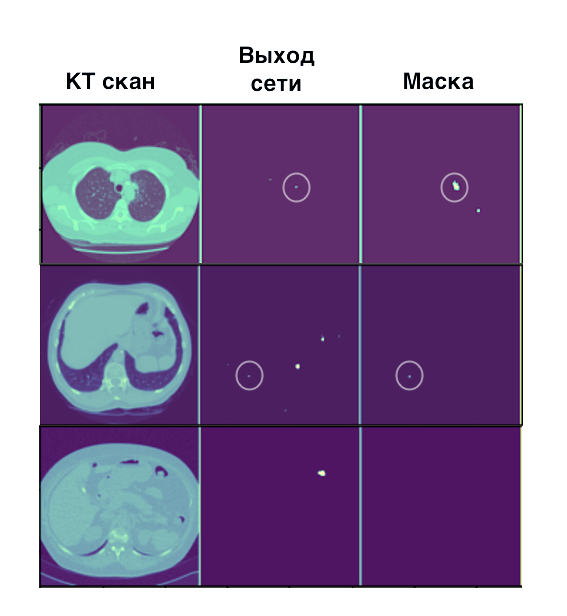
\includegraphics[width=\linewidth]{images/2d-seg-results.png}
\caption{Результаты работы сети}\label{mirskiy-cgan-architecture}
\centering
\end{figure}

Кругом обозначены совпадения на выходе сети и на истинной маске. На нижнем примере видно, что сеть ошибочно распознала участок ткани визуально похожий на опухоль, но в реальности ею не являющийся.

\section{Выводы по главе 2}

Полученные результаты явно свидетельствуют о непригодности использования подобных $end-to-end$ технологий для сегментации $2d$ изображений. Предполагаемое объяснение состоит в том, что двухмерные сканы не в состоянии передать достаточный набор признаков, позволяющий отличить опухоль от другого, похожего на нее участка легкого. Дело в том, что каждый двухмерный слайс содержит только лишь срез трехмерной опухоли, и значительная часть таких срезов может иметь вполне неопределенную форму, ничем не отличимую от сосудов в легких. Отсюда следует большая необходимость в использовании трехмерных зависимостей между различными слайсами для решения задачи распознавания.

